\chapter{Backup}
\label{chap:Backup}

\section{Dilepton Plots with \mediumPP\ Electrons}
\graphicspath{{Chapters/ObjEventSelection/Figures}}

\begin{figure}[h]
\centering
	\subfigure[]{
            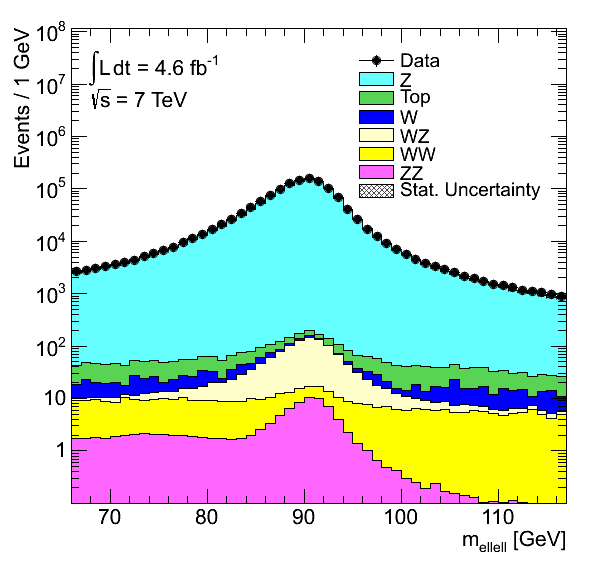
\includegraphics[width=0.47\textwidth]{Dilepton7TeV/CeECeE_pt20MediumPP_Z_m}
        }
	\subfigure[]{
            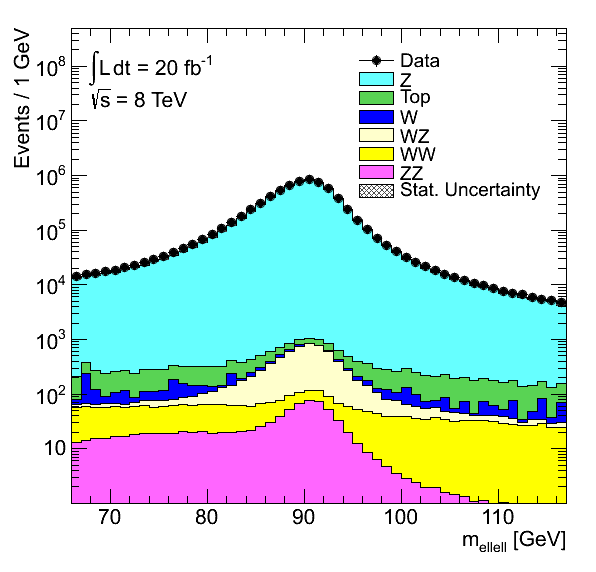
\includegraphics[width=0.47\textwidth]{Dilepton8TeV/CeECeE_pt20MediumPP_Z_m}
        }
	\subfigure[]{
            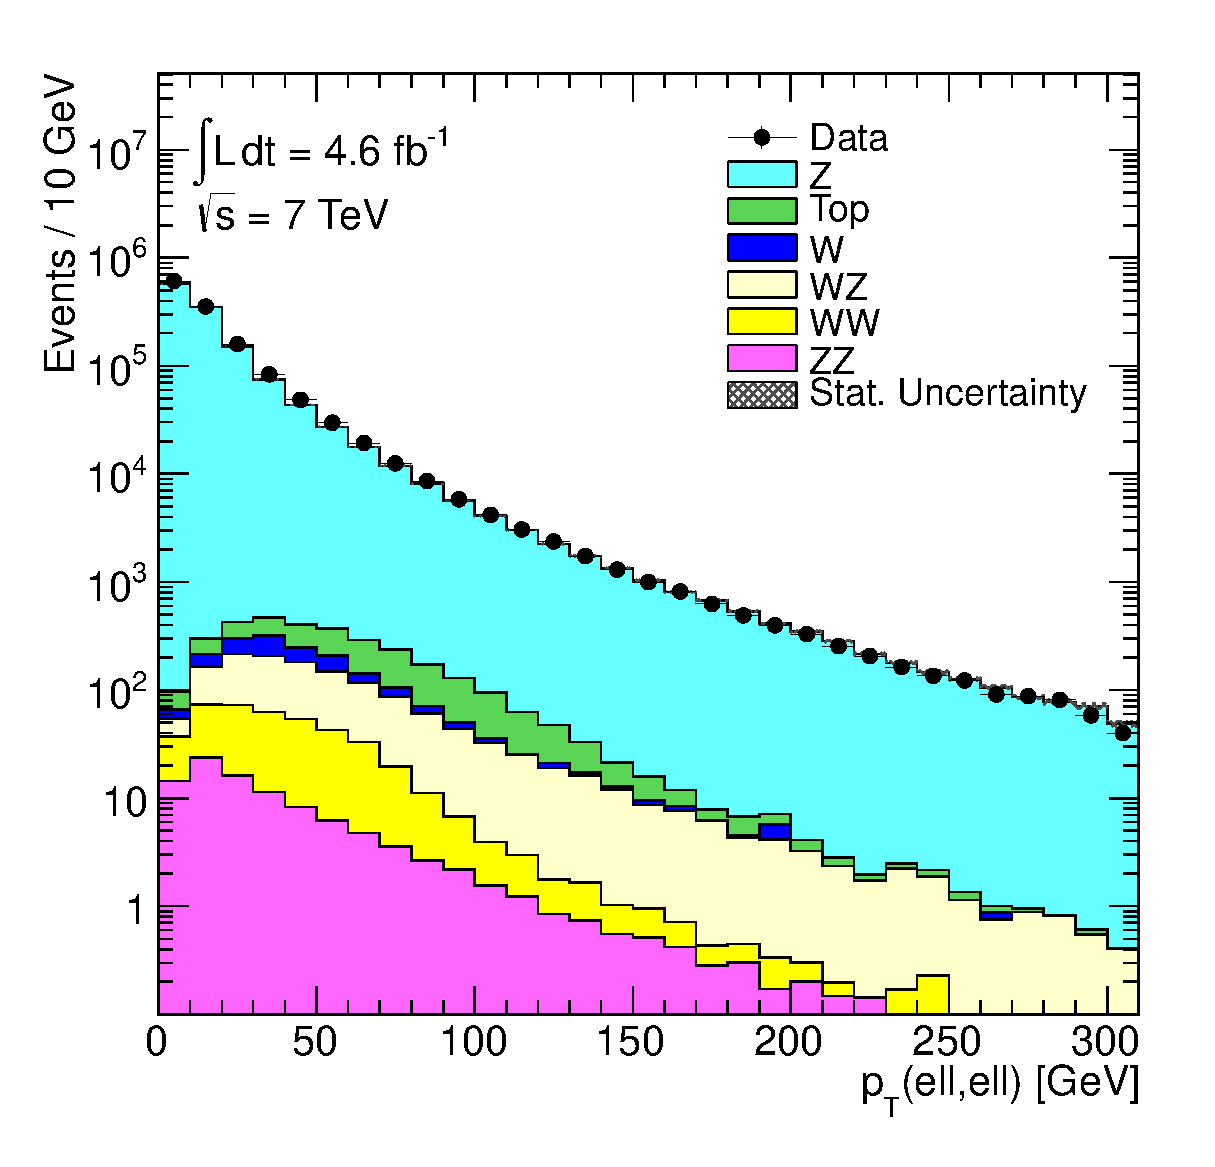
\includegraphics[width=0.47\textwidth]{Dilepton7TeV/CeECeE_pt20MediumPP_Z_pt}
        }
	\subfigure[]{
            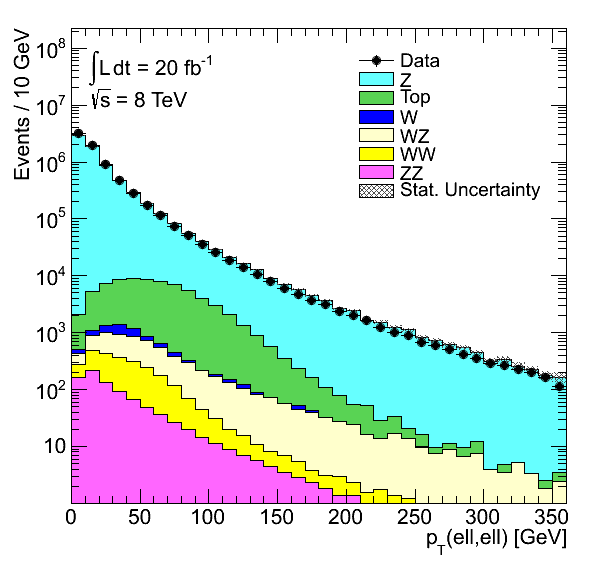
\includegraphics[width=0.47\textwidth]{Dilepton8TeV/CeECeE_pt20MediumPP_Z_pt}
        }
    \caption[Dilepton invariant mass and transverse momentum in the 7~\tev\
    data. ]
    {Figures (a) and (b) show distributions of the \dilepton\ invariant mass for \dielectron\ and 
     \dimuon\ pairs, respectively, in events in the 7~\tev\ data containing a pair of
    \ossf\ leptons passing all of the lepton selection criteria described
    in Sections~\ref{sec:objsel-el} and~\ref{sec:objsel-mu}. Figures (c) and (d) show the \dilepton\ transverse momentum for
    events passing the same criteria, with the additional requirement that the
    \dilepton\ pair have \sstooos. 
    }
\label{fig:dilep-mass-pt-seven}
\end{figure}

\begin{figure}[h]
\centering
\vspace{-5mm}
	\subfigure[]{
            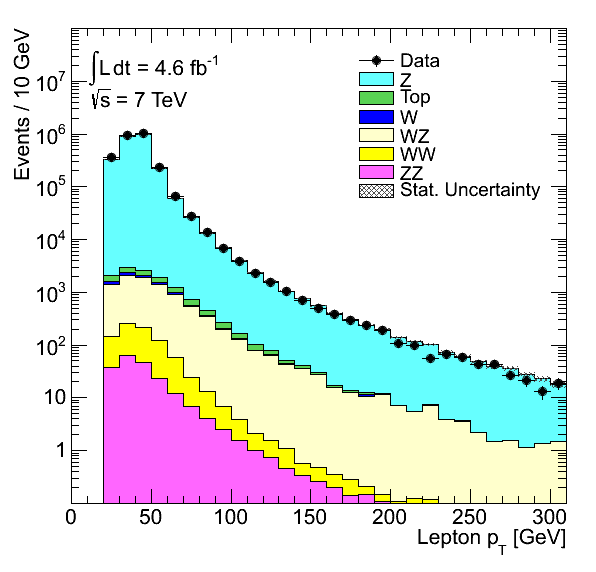
\includegraphics[width=0.47\textwidth]{Dilepton7TeV/CeECeE_pt20MediumPP_lep_pt}
        }
	\subfigure[]{
            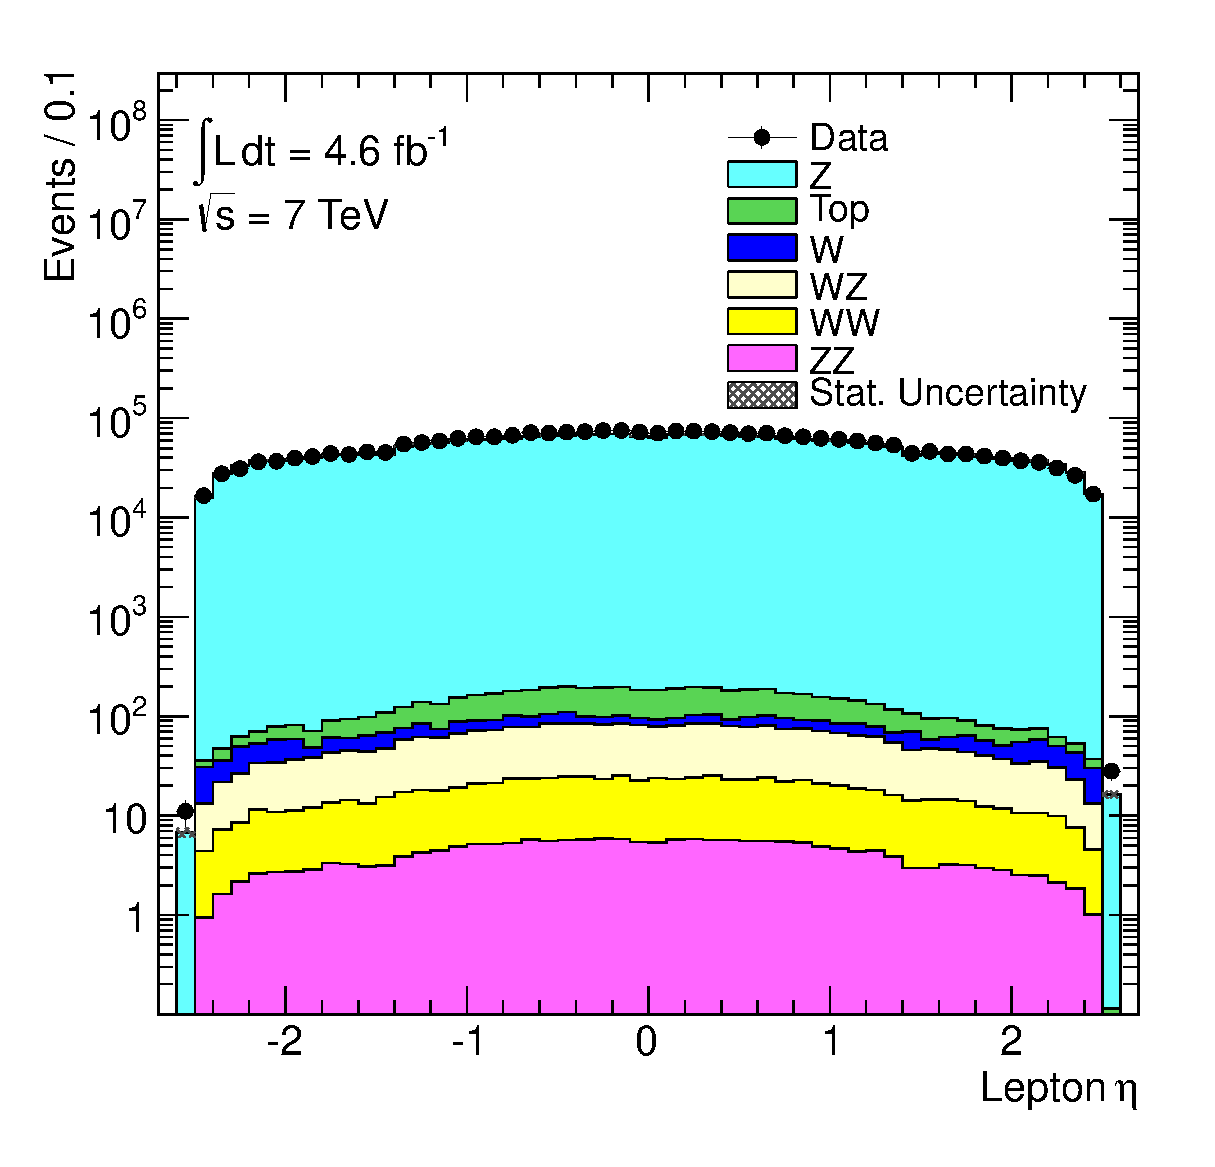
\includegraphics[width=0.47\textwidth]{Dilepton7TeV/CeECeE_pt20MediumPP_lep_eta}
        }
	\subfigure[]{
            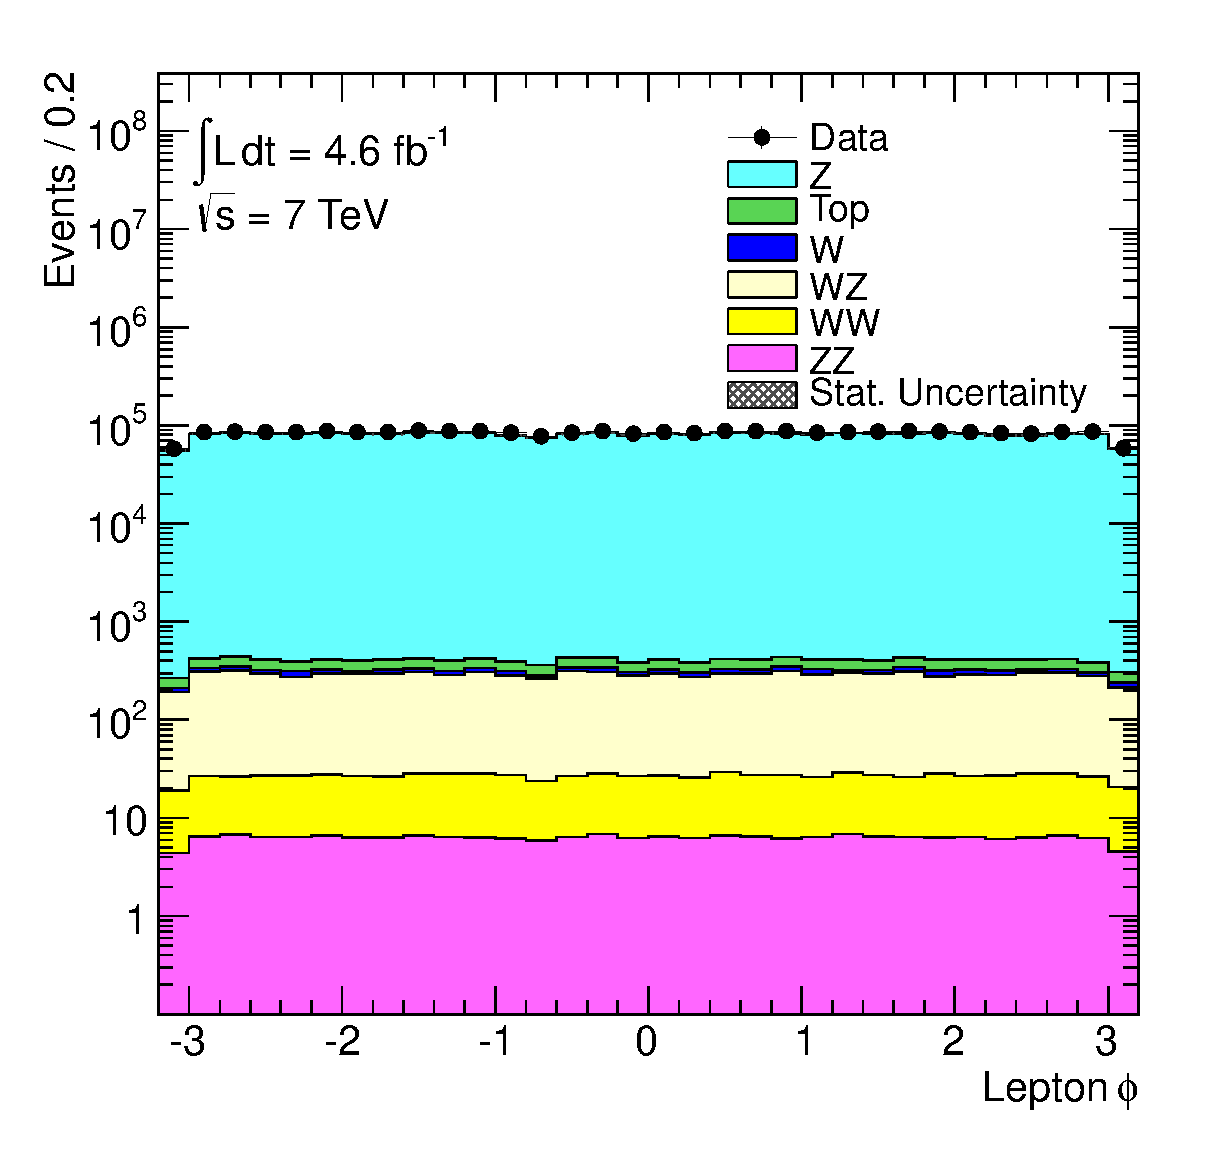
\includegraphics[width=0.47\textwidth]{Dilepton7TeV/CeECeE_pt20MediumPP_lep_phi}
        }
    \caption[Lepton kinematic distributions for \dilep\ events in the 7~\tev\
    data. ]
    {\small Kinematic distributions for leptons in events in the 7~\tev\
    data containing an \ossf\ lepton pair. The leptons are required to pass all of the selection
    requirements described in Sections~\ref{sec:objsel-el}
    and~\ref{sec:objsel-mu} and the pair must have \sstooos. 
    Figures (a) and (b) show the lepton \pt\ for electrons and muons
    respectively, figures (c) and (d) the lepton $\eta$ and figures (d) and (e)
    the lepton $\phi$.    }
\label{fig:dilep-lepkin-seven}
\end{figure}
